\section{Реализация алгоритма}
\label{}

Требования, предъявленные к разрабатываемому исполняемому файлу:
\begin{enumerate}
\item Время исполнения для предоставленных файлов-примеров имеет порядок секунд или минут. Возможность работы в реальном времени не требуется.
\item Целевая платформа --- Microsoft Windows. Доступны инструменты .NET Framework.
\item Графический интерфейс не требуется, т.к. взаимодействие программы с пользователем минимально.
\end{enumerate}

Кроме того, для работы с большими массивами структур данных требуются инструменты высокого уровня. Исходя из этих требований, для реализации алгоритма был выбран язык C\#: он полностью поддерживается платформой .NET Framework и обладает высокоуровневым инструментарием LINQ. В качестве среды разработки выбрана Microsoft Visual Studio 2013.

\subsection{Интерфейс}
\label{}

Выбор файлов для обработки реализован при помощи вызова системного диалога Windows через класс OpenFileDialog .NET Framework. После этого вывод отладочной информации осуществляется через текстовый интерфейс.

\begin{figure}[!htb]
    \centering
    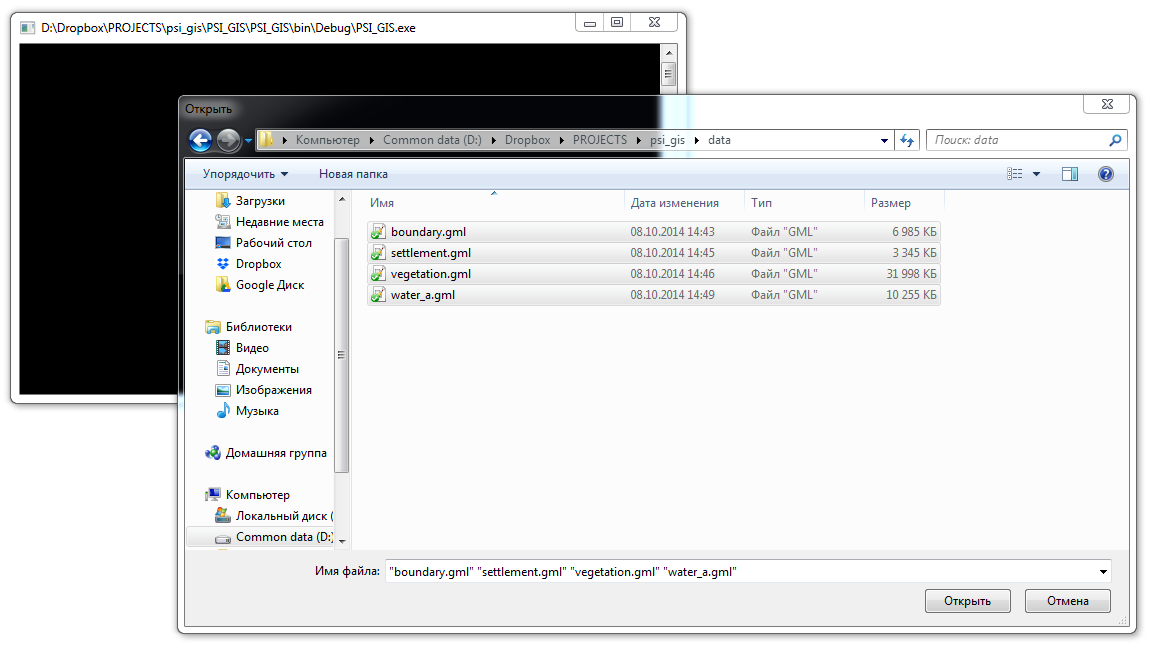
\includegraphics[width=1\textwidth]{dialog.png}
    \caption{Интерфейс ввода данных}
    \label{fig:dialog}
\end{figure}

\subsection{Объектная модель данных}
\label{}



\subsection{Пример работы}
\label{}

См. рис. \ref{fig:nocuts} и \ref{fig:result}.

\begin{figure}[!htb]
    \centering
    
\includegraphics[width=1\textwidth]{nocuts.png}
    \caption{Визуализация фрагмента входного файла}
    \label{fig:nocuts}
\end{figure}

\begin{figure}[!htb]
    \centering
    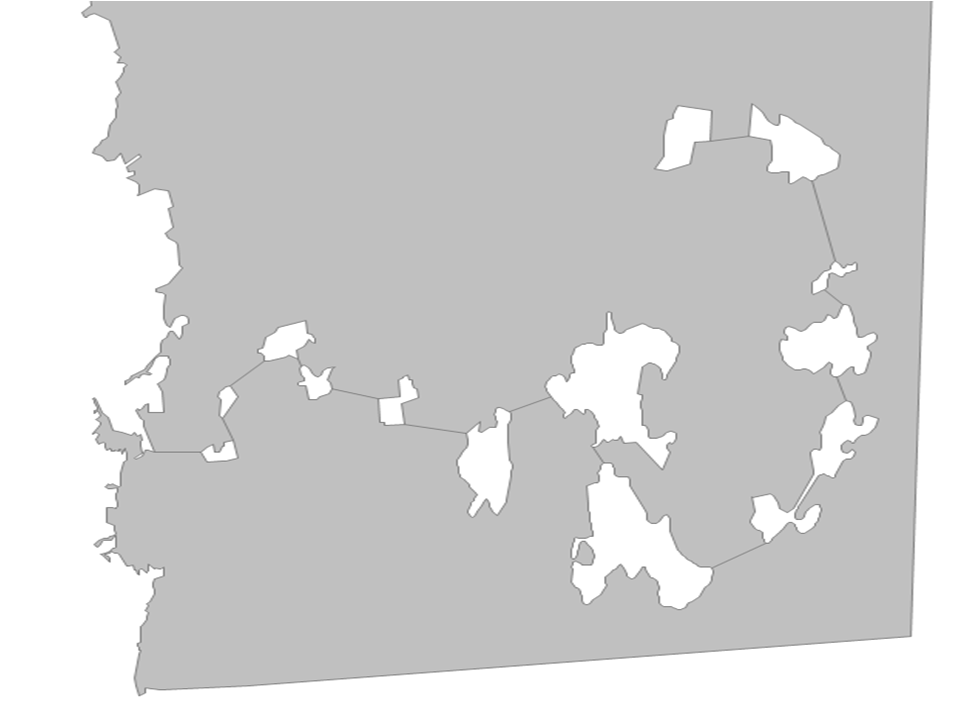
\includegraphics[width=1\textwidth]{result.png}
    \caption{Результат преобразования фрагмента файла}
    \label{fig:result}
\end{figure}